%%%%%%%%%%%%%%%%%%%%%%%%%%%%%%%%%%%%%%%%%
% Energy modelling outreach course
% Version 0.1 (2022-01)

%
% Author:
% Leonhard Hofbauer
%
% based on the kaobook class (LPPL 1.3) and respective template (CC0) by Federico Marotta
%%%%%%%%%%%%%%%%%%%%%%%%%%%%%%%%%%%%%%%%%

%----------------------------------------------------------------------------------------
%	PACKAGES AND OTHER DOCUMENT CONFIGURATIONS
%----------------------------------------------------------------------------------------

\documentclass[
	fontsize=10pt, % Base font size
	twoside=false, % Use different layouts for even and odd pages (in particular, if twoside=true, the margin column will be always on the outside)
	%open=any, % If twoside=true, uncomment this to force new chapters to start on any page, not only on right (odd) pages
	%chapterprefix=true, % Uncomment to use the word "Chapter" before chapter numbers everywhere they appear
	%chapterentrydots=true, % Uncomment to output dots from the chapter name to the page number in the table of contents
	numbers=noenddot, % Comment to output dots after chapter numbers; the most common values for this option are: enddot, noenddot and auto (see the KOMAScript documentation for an in-depth explanation)
	%draft=true, % If uncommented, rulers will be added in the header and footer
	%overfullrule=true, % If uncommented, overly long lines will be marked by a black box; useful for correcting spacing problems
]{kaobook}

% Set the language
\usepackage[english]{babel} % Load characters and hyphenation
\usepackage[english=british]{csquotes} % English quotes

% Load packages for testing
\usepackage{blindtext}
%\usepackage{showframe} % Uncomment to show boxes around the text area, margin, header and footer
%\usepackage{showlabels} % Uncomment to output the content of \label commands to the document where they are used

% Load the bibliography package
\usepackage{styles/kaobiblio}
\addbibresource{main.bib} % Bibliography file

% Load mathematical packages for theorems and related environments. NOTE: choose only one between 'mdftheorems' and 'plaintheorems'.
\usepackage{styles/mdftheorems}
%\usepackage{styles/plaintheorems}

\graphicspath{{examples/documentation/images/}{files/}} % Paths in which to look for images

\makeindex[columns=3, title=Alphabetical Index, intoc] % Make LaTeX produce the files required to compile the index

\makeglossaries % Make LaTeX produce the files required to compile the glossary

\makenomenclature % Make LaTeX produce the files required to compile the nomenclature

% Reset sidenote counter at chapters
%\counterwithin*{sidenote}{chapter}

%----------------------------------------------------------------------------------------

\begin{document}

%----------------------------------------------------------------------------------------
%	BOOK INFORMATION
%----------------------------------------------------------------------------------------

%\titlehead{The \texttt{kaobook} class}
\subject{\texttt{A short course}}

\title[Energy system modelling]{Can wind power society? How we use computer tools to plan our energy future}
%\subtitle{Customise this page according to your needs}

\author[Leonhard Hofbauer]{}

\date{}%\today

\publishers{}%University College London

%----------------------------------------------------------------------------------------

\frontmatter % Denotes the start of the pre-document content, uses roman numerals

%----------------------------------------------------------------------------------------
%	OPENING PAGE
%----------------------------------------------------------------------------------------

%\makeatletter
%\extratitle{
%	% In the title page, the title is vspaced by 9.5\baselineskip
%	\vspace*{9\baselineskip}
%	\vspace*{\parskip}
%	\begin{center}
%		% In the title page, \huge is set after the komafont for title
%		\usekomafont{title}\huge\@title
%	\end{center}
%}
%\makeatother

%----------------------------------------------------------------------------------------
%	COPYRIGHT PAGE
%----------------------------------------------------------------------------------------

\makeatletter
\uppertitleback{\@titlehead} % Header

\lowertitleback{
	\textbf{Version} \\
	This is version 0.1 of the course handbook.
	
	\medskip
	
	\textbf{Copyright}\\
	\ccby\ This document is \textcopyright Leonhard Hofbauer, 2022, and is released under the CC-BY-4.0 license. 
	
	To view a copy of the license, visit: \\\url{https://creativecommons.org/licenses/by/4.0/}
	\medskip
	
	\textbf{Acknowledgements} \\
	The author is grateful for the support provided by the \href{https://thebrilliantclub.org/}{The Brilliant Club} during the preparation of an earlier version of this handbook.
	
		
	\medskip
	
	\textbf{Colophon} \\
	This document was typeset with the help of \href{https://sourceforge.net/projects/koma-script/}{\KOMAScript} and \href{https://www.latex-project.org/}{\LaTeX} using the \href{https://github.com/fmarotta/kaobook/}{kaobook} class.
	

	

}
\makeatother

%----------------------------------------------------------------------------------------
%	DEDICATION
%----------------------------------------------------------------------------------------

%\dedication{
%}

%----------------------------------------------------------------------------------------
%	OUTPUT TITLE PAGE AND PREVIOUS
%----------------------------------------------------------------------------------------

% Note that \maketitle outputs the pages before here

% If twoside=false, \uppertitleback and \lowertitleback are not printed
% To overcome this issue, we set twoside=semi just before printing the title pages, and set it back to false just after the title pages
\KOMAoptions{twoside=semi}
\maketitle
\KOMAoptions{twoside=false}

%----------------------------------------------------------------------------------------
%	PREFACE
%----------------------------------------------------------------------------------------

%\chapter*{Preface}
%\addcontentsline{toc}{chapter}{Preface} % Add the preface to the table of contents as a chapter

% TODO: potentialy add personal statement/acknowledgements here



\section*{Course summary}

Energy powers societies all around the world. From mobile phones, to cars, to cook stoves, people use the earth's energy resources, for example crude oil or the energy in wind, to enhance their lifestyles. But these energy systems are also connected to some of the major challenges we are facing at the moment: the climate crisis, air pollution, and providing access to energy for all people all around the world. In order to address these challenges, we need to change the way we source and use energy, so the energy system is environmentally and socially sustainable.\\

In this course, we will learn how we can use computer tools, so-called energy system models, to help us plan a transition to a sustainable energy system. In the first two sessions, we will discuss the energy system and energy system models in general. Afterwards, we will look in more detail at particular techniques used to build and operate these tools. You will also be given a base model and use it yourself to answer questions about how we can generate the electricity we need in future. Based on our discussions and your experience with the model, we will also have a critical look at the strengths and weaknesses of these tools.\\

This course will give you the chance to develop a good understanding of how we use energy, what challenges are related to this, and how to use energy models to address questions about future solutions. It will help you to think more critically about things you hear and read and how to write down your thoughts more precisely.\\

\section*{Course structure}

The course consists of 5 sessions, each including homework that is an integral part of the course. Each session has a separate section in this handbook providing relevant material and tasks. The final coursework will be introduced in session 5 and gives you the opportunity to work independently on your own scientific energy analysis.

%----------------------------------------------------------------------------------------
%	TABLE OF CONTENTS & LIST OF FIGURES/TABLES
%----------------------------------------------------------------------------------------

\begingroup % Local scope for the following commands

% Define the style for the TOC, LOF, and LOT
%\setstretch{1} % Uncomment to modify line spacing in the ToC
%\hypersetup{linkcolor=blue} % Uncomment to set the colour of links in the ToC
\setlength{\textheight}{23cm} % Manually adjust the height of the ToC pages

% Turn on compatibility mode for the etoc package
\etocstandarddisplaystyle % "toc display" as if etoc was not loaded
\etocstandardlines % toc lines as if etoc was not loaded

\tableofcontents % Output the table of contents

\listoffigures % Output the list of figures

% Comment both of the following lines to have the LOF and the LOT on different pages
\let\cleardoublepage\bigskip
\let\clearpage\bigskip

\listoftables % Output the list of tables

\endgroup

%----------------------------------------------------------------------------------------
%	MAIN BODY
%----------------------------------------------------------------------------------------

\mainmatter % Denotes the start of the main document content, resets page numbering and uses arabic numbers
\setchapterstyle{kao} % Choose the default chapter heading style
%\setchapterpreamble[u]{\margintoc}
\chapter{Introduction}
\labch{intro}

% TODO: add more general course information, e.g., marking scheme, here.

\setchapterpreamble[u]{\margintoc}
\chapter{Energy Systems}
\labch{tut1}


After completing this session successfully, you should be able

\begin{itemize}
\item to understand what an energy system is,
\item to know about issues connected with current energy systems, and
\item to explain the necessity of energy system transitions.
\end{itemize}


\section{What is an energy system?}

\paragraph*{Defining energy and energy system.}

\begin{kaobox}[frametitle=Task]
What do you think about when you hear the word \textit{energy}? What do you think an \textit{energy system} is?
\end{kaobox}

\begin{definition}
\labdef{energy}
Energy is the capacity for doing work. It can exist in potential, kinetic, thermal, chemical, and various other forms \sidecite{britannica_the_editors_of_encyclopaedia_energy_nodate}.
\end{definition}

\begin{definition}
\labdef{es}
The energy system encompasses all components involved in the production, conversion, delivery, and use of energy \sidecite{intergovernmental_panel_on_climate_change_climate_2014}.
\end{definition}

It is important to have in mind that the whole purpose of the energy system is to fulfil the demand for energy services to satisfy human needs. Thus, the energy system is also sometimes defined as all arrangements whereby humans make use of the Earth’s energy resources to enhance their lives \sidecite{smil_energy_2010}.

% TODO: add a side note on what energy resources are (including fossil, renewable examples, etc.)

\paragraph*{Understanding what is part of the energy system.}

\begin{kaobox}[frametitle=Task]
Look at the photos in \reffig{es_photos}, what do you think is part of the energy system? Can you identify different types of elements of the energy system?
\end{kaobox}

\begin{figure}[hb]
	\includegraphics[height=0.34\textwidth]{files/ES_photo_1.jpg}
	\includegraphics[height=0.34\textwidth]{files/ES_photo_2.jpg}\\
	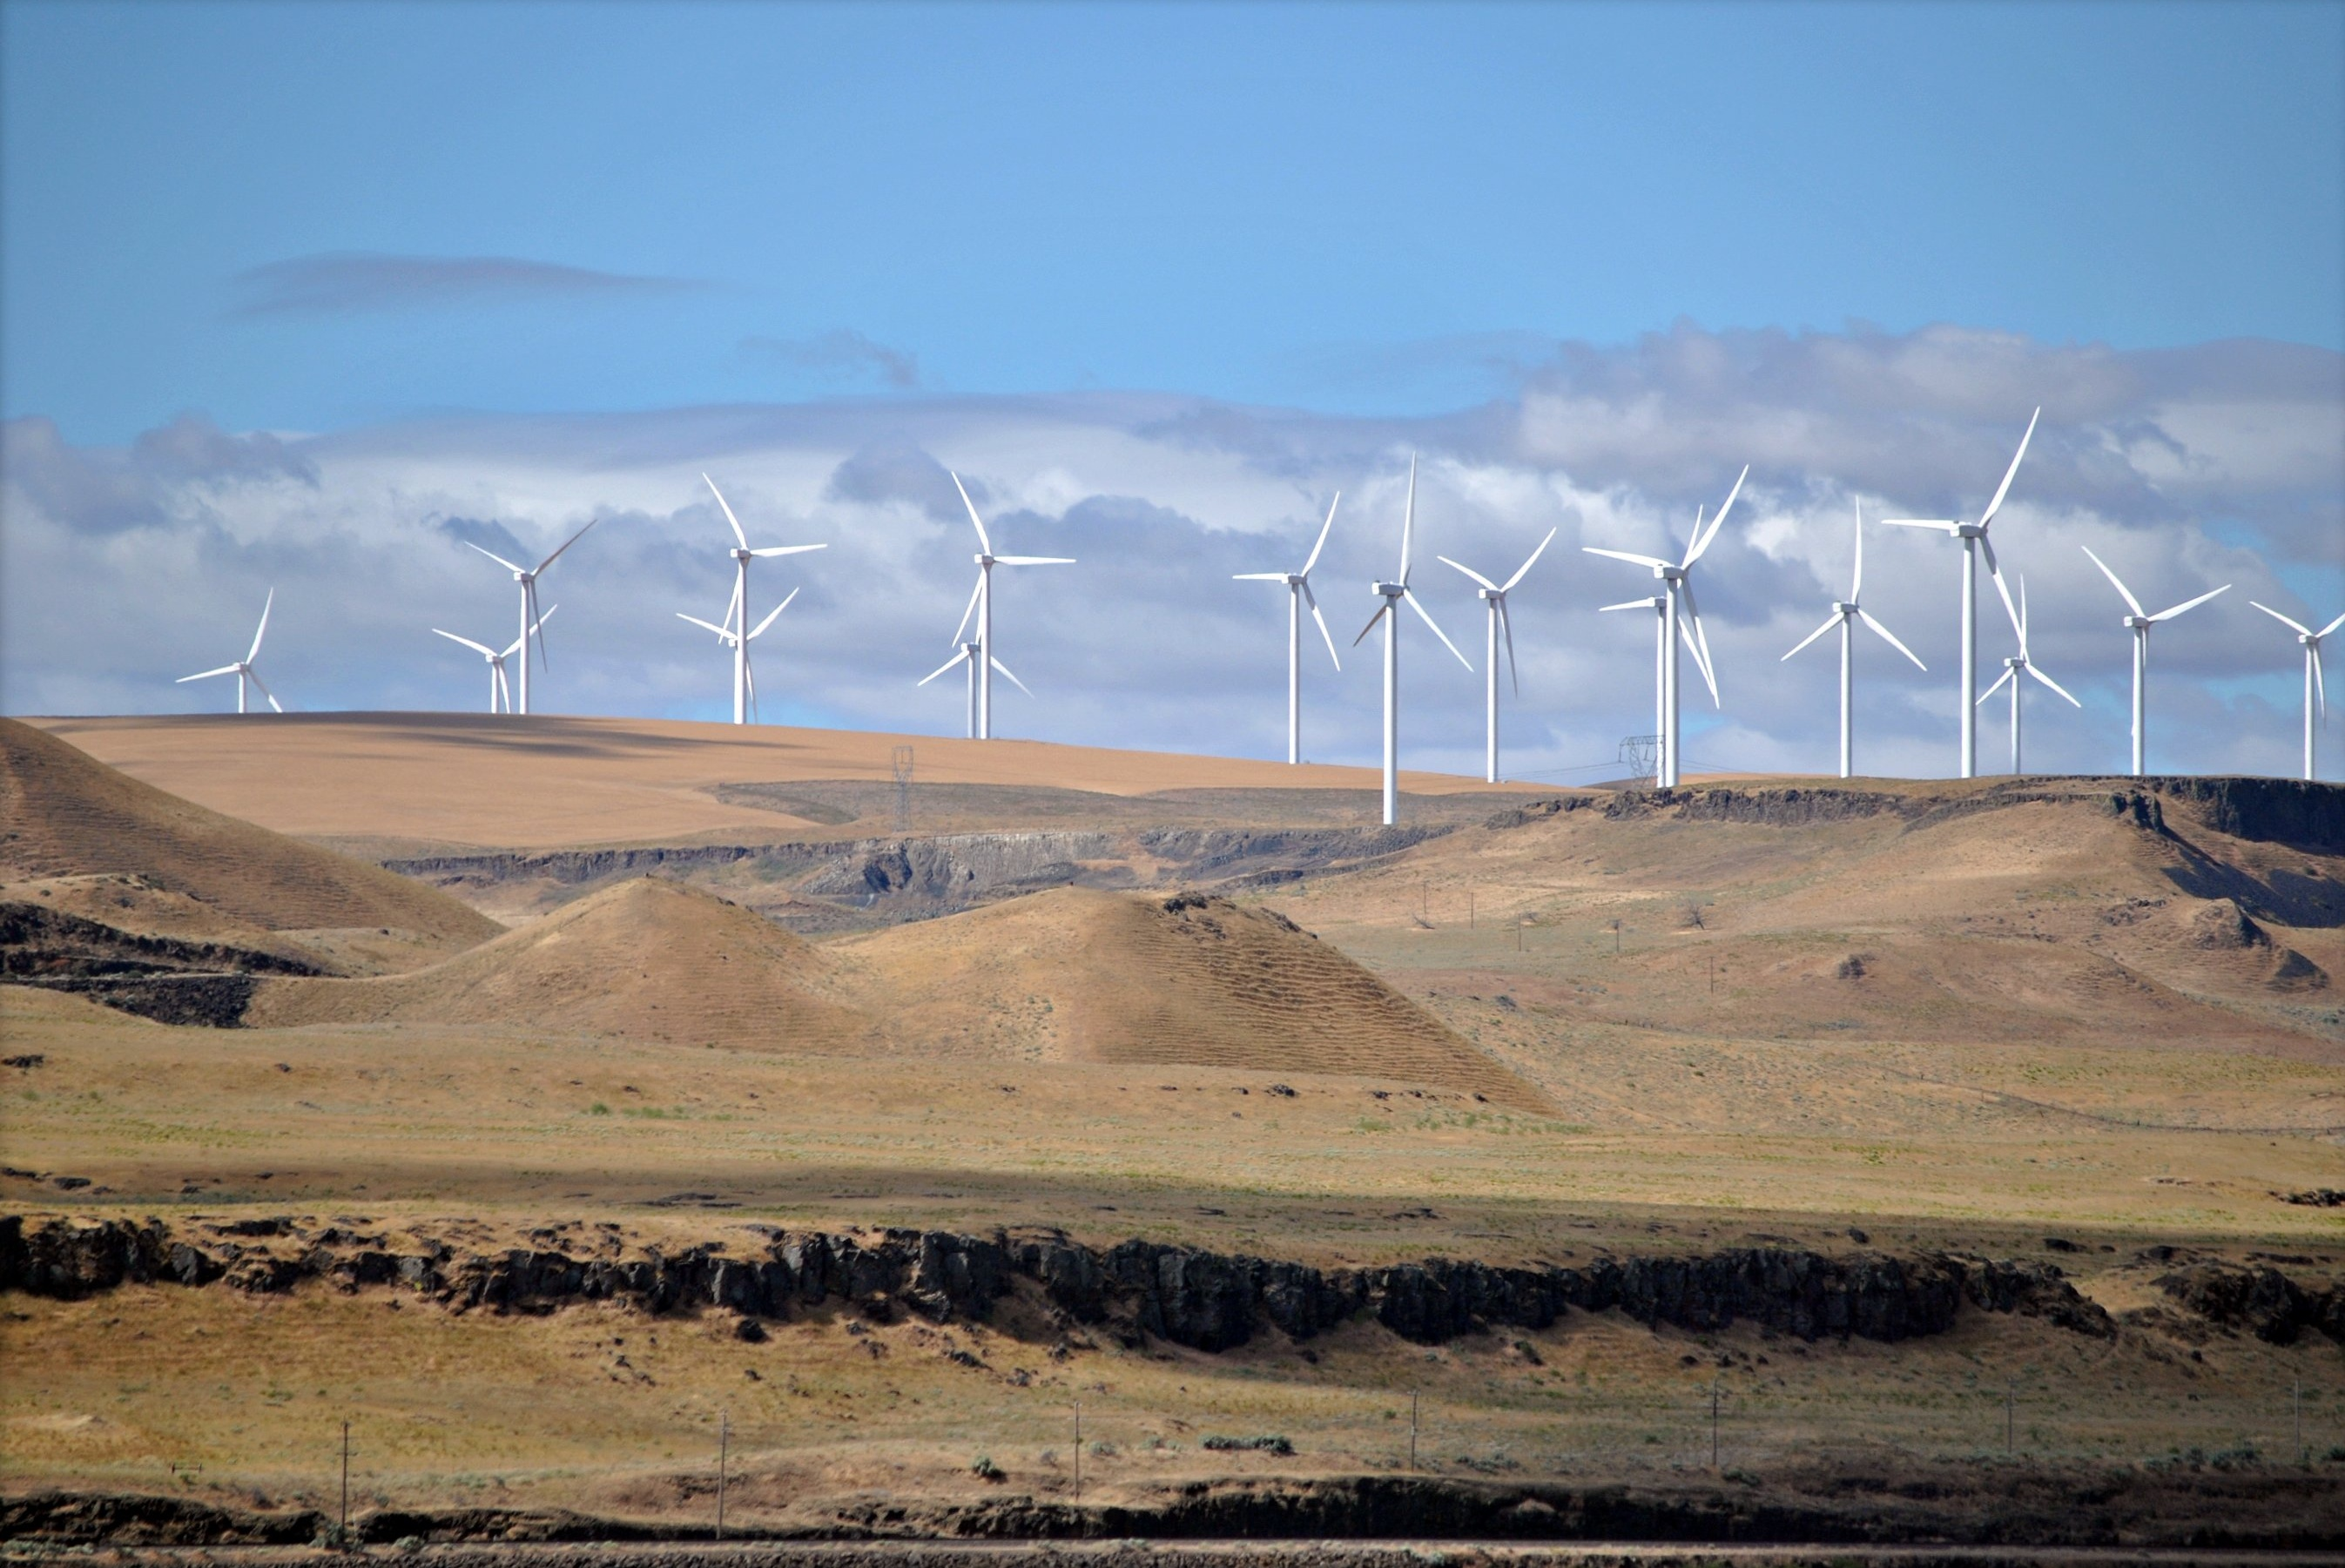
\includegraphics[height=0.34\textwidth]{files/ES_photo_3.jpg}
	\includegraphics[height=0.34\textwidth]{files/ES_photo_4.jpg}
	\caption[Photos showing different parts of the energy system.]{Photos showing different parts of the energy system. Bottom right photo, \copyright Leonhard Hofbauer, 2021, released under a CC-BY-4.0, the remaining photos, clockwise, are from Steve Wilson, VasenkaPhotography, and Stig Nygaard, respectively, and all licensed under a CC-BY-2.0.}
\labfig{es_photos}
\end{figure}


 
\section{Major issues of current energy systems}
\labsec{issues}

\paragraph*{Considering problems connected to current energy systems.}

\begin{kaobox}[frametitle= Excerpt from \sidecite{maciel_energy_2012} (reprinted under a CC-BY-4.0), backgroundcolor=Goldenrod!45!white,frametitlebackgroundcolor=Goldenrod!45!white]
Worldwide, transportation generates over 23\% of the total of greenhouse gas emissions arising from the use of energy and accounts for at least 26\% of the planet's energy consumption [1,2,3,4,5,6]. The transportation sector occupies between 15\% and 25\% of the land mass in major cities throughout the World [7,8,9,10,11], and the time lost in traffic congestion in several countries leads to an economic loss of approximately 1 to 3\% of GDP [12].\\

Furthermore, over a million people die and three million are injured every year in road traffic accidents worldwide [13,14,15]. These accidents result in economic costs of approximately 5\% of GDP in some countries [16]. Several countries considered to be `emerging' economically, such as Brazil, have adopted transportation systems that repeat the errors committed by more developed countries, including the encouragement of individual motorized transportation as the standard model. This has not proved to be the optimal solution [17].\\

Additionally, studies on the causes of persistent poverty in the peripheral areas of large cities, both in developed and emerging countries, point to a lack of transportation as one of the principal causes of social ills [18]. It is clear that an economy suffers significant losses in the absence of adequate transportation support. A sustainable transportation strategy has the potential to make a significant contribution to the environmental, economic and social development of cities and surrounding areas [19].\\

In Brazil, where the government regularly proclaims its overriding commitment to both the efficient use of public resources and the improvement of living standards for the population, there is an urgent and evident need for a drastic overhaul of the currently unsustainable transportation system. An accurate and reliable projection of the consumption of resources and the level of emissions produced by our transportation system in the coming decades is a key factor in ensuring the adequate redirection of public policies and the consequent benefits to the population.
\end{kaobox}

\begin{kaobox}[frametitle=Task]
Read through the box above, which talks about the transport sector, a part of the energy system. What issues related to the current transport system are mentioned? Are these issues also existing more widely in other parts of the energy system? Can you think of any other issues connected to the current transport and energy system not mentioned in the text?
\end{kaobox}

\section{The energy transition}

\paragraph*{The need for energy transitions.}~\\

% TODO: add a definition and/or more information on the energy transition in a side note

The issues discussed in the previous section -- climate change, pollution, health impacts, energy poverty, and others -- require that we change the way societies extract, transport, and use energy. This is often described as energy transition.

\begin{kaobox}[frametitle=Task]
Who do you think is responsible for the energy transition? Why?
\end{kaobox}


\section{Homework}
\labsec{hw1}

\begin{figure}[hb]
	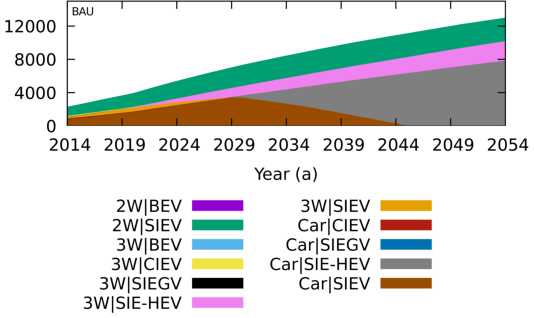
\includegraphics[width=0.95\textwidth]{files/india_transport.pdf}
	\caption[Transport sector pathway for India.]{Graph showing the passenger transport performance in billion person kilometres (bpkm) for a potential pathway for the Indian road transport system (2W: motorcycle, 3W: 3-wheeler motorcycle, BEV: battery electric vehicle, CIEV: diesel vehicle, FCV: fuel cell hydrogen vehicle, HEV: hybrid electric vehicle, SIEGV: CNG/gas vehicle, SIEV: petrol vehicle). Adopted from \cite{hofbauer_shaping_2018}.}
	\labfig{india_transport}
\end{figure}


\reffig{india_transport} above shows how the road transport sector in India might develop in future. It was part of a study that described several of those possible future pathways.

Write a text that covers the following three elements:
\begin{itemize}
\item Write a short description the development shown in the figure.
\item Research and discuss one or two social or environmental problems of the energy system in India at the moment and explain how this development could worsen or improve these problems.
\item Describe changes one could make to this development to solve these issues.
\end{itemize}


Please have the following points in mind when working on your assignment:

\begin{itemize}
\item Your assignment needs to be 500 $\pm$ 10\% words long.
\item You need to submit your assignment on the platform and before the deadline mentioned by your course leader.
\item If you have any questions while working on the assignment, do not hesitate to approach your course leader.
\end{itemize}
\setchapterpreamble[u]{\margintoc}
\chapter{Energy System Modelling}
\labch{esm}


After completing this session successfully, you should be able

\begin{itemize}
\item to understand what a model is,
\item to understand the purpose of energy system models, and
\item to know about different characteristics of energy models.
\end{itemize}



\section{What are models?}
\labsec{models}


\paragraph*{Defining what a model is.}

\begin{kaobox}[frametitle=Task]
Have a look again at the task description for the homework of session 1 (Section \ref{sec:hw1}). How do you think the graph showing the future development was created?
\end{kaobox}


There are many different ways of defining what a model is. One widely used, general definition of a model has been developed by a researcher called Stachowiak \sidecite{stachowiak_allgemeine_1973}. He defines models by describing three important characteristics every model needs to fulfil. \refdef{model} lists all three characteristics.

\begin{definition}
\labdef{model}
Every model has three characteristics. A model
\begin{itemize}
\item  is always a model \textbf{of something}, i.e., it is a representation or depiction of a material or immaterial original,
\item is a simplification, i.e., does not have all attributes the original object has, and
\item aims to fulfil a particular purpose or function for the people building and/or using it.
\end{itemize}
\end{definition}

In short, a model is a simplified depiction of an original, built and used for a particular purpose. Such models can look very different and can have very different purposes. One example for a model is a physical miniature model of a building used by an architect to showcase the building design. The model is a depiction of an original building, either an existing building or a potential future building (characteristic 1). It is much smaller than the original and lacks a lot of the more detailed features, e.g., water pipes and furniture, and, thus, is a simplified representation of the original (characteristic 2). The model aims to fulfil a particular purpose, i.e., showcasing the architect's design to a project developer -- at the same time, it is inadequate to, for example, study the thermal performance of the original because it is built from very simple materials (characteristic 3). Another example would be a computer-based model of a chemical molecule that can be used by a chemist to predict the chemical properties of the molecule.


\paragraph*{Different kind of models.}~\\

Based on the definition from above, there is a wide range of different kind of models.

\begin{kaobox}[frametitle=Task]
Have a look at the pictures in \reffig{model_photos}. Which of those shows a) a model, b) an energy system model in particular, or c) no model at all? Explain your decisions.
\end{kaobox}

\begin{figure}[hb]
	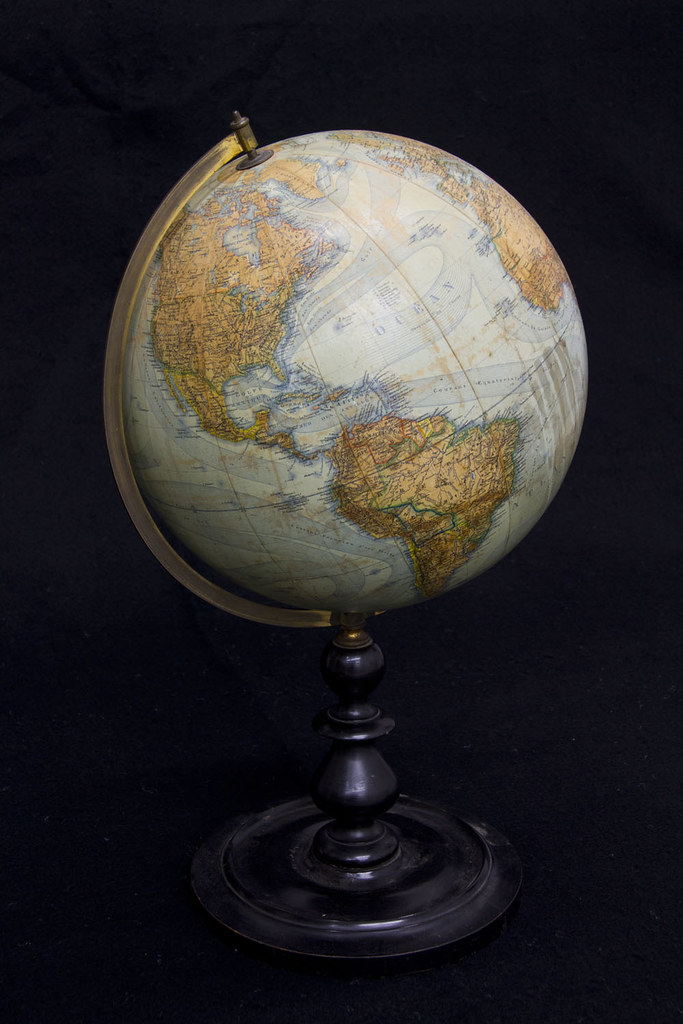
\includegraphics[height=0.38\textwidth]{files/Model_photo_1.jpg}
	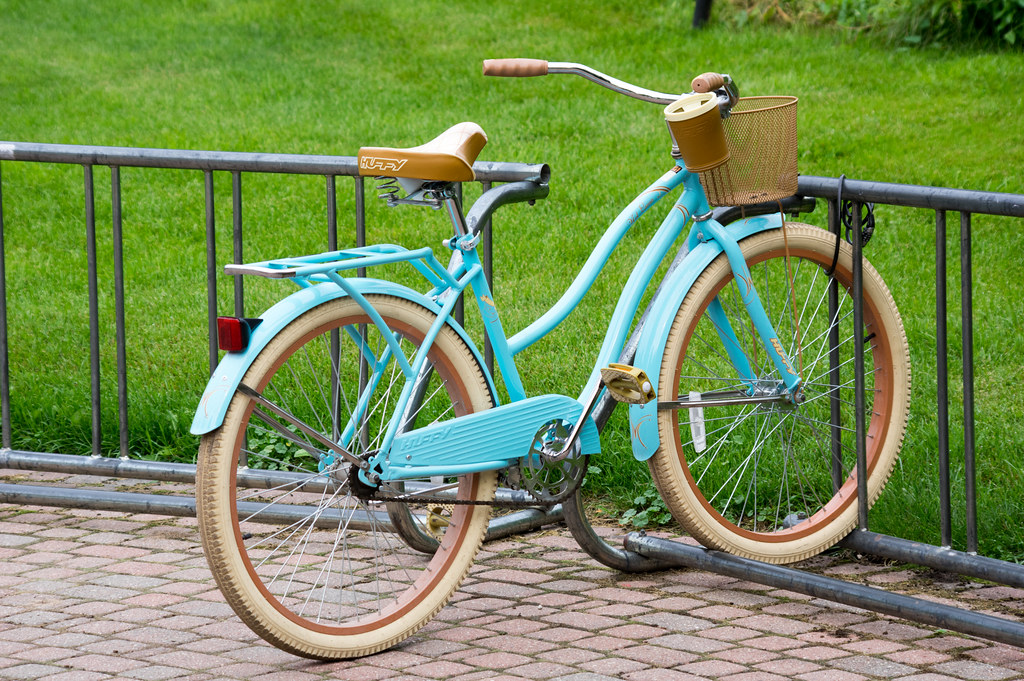
\includegraphics[height=0.38\textwidth]{files/Model_photo_2.jpg}\\
	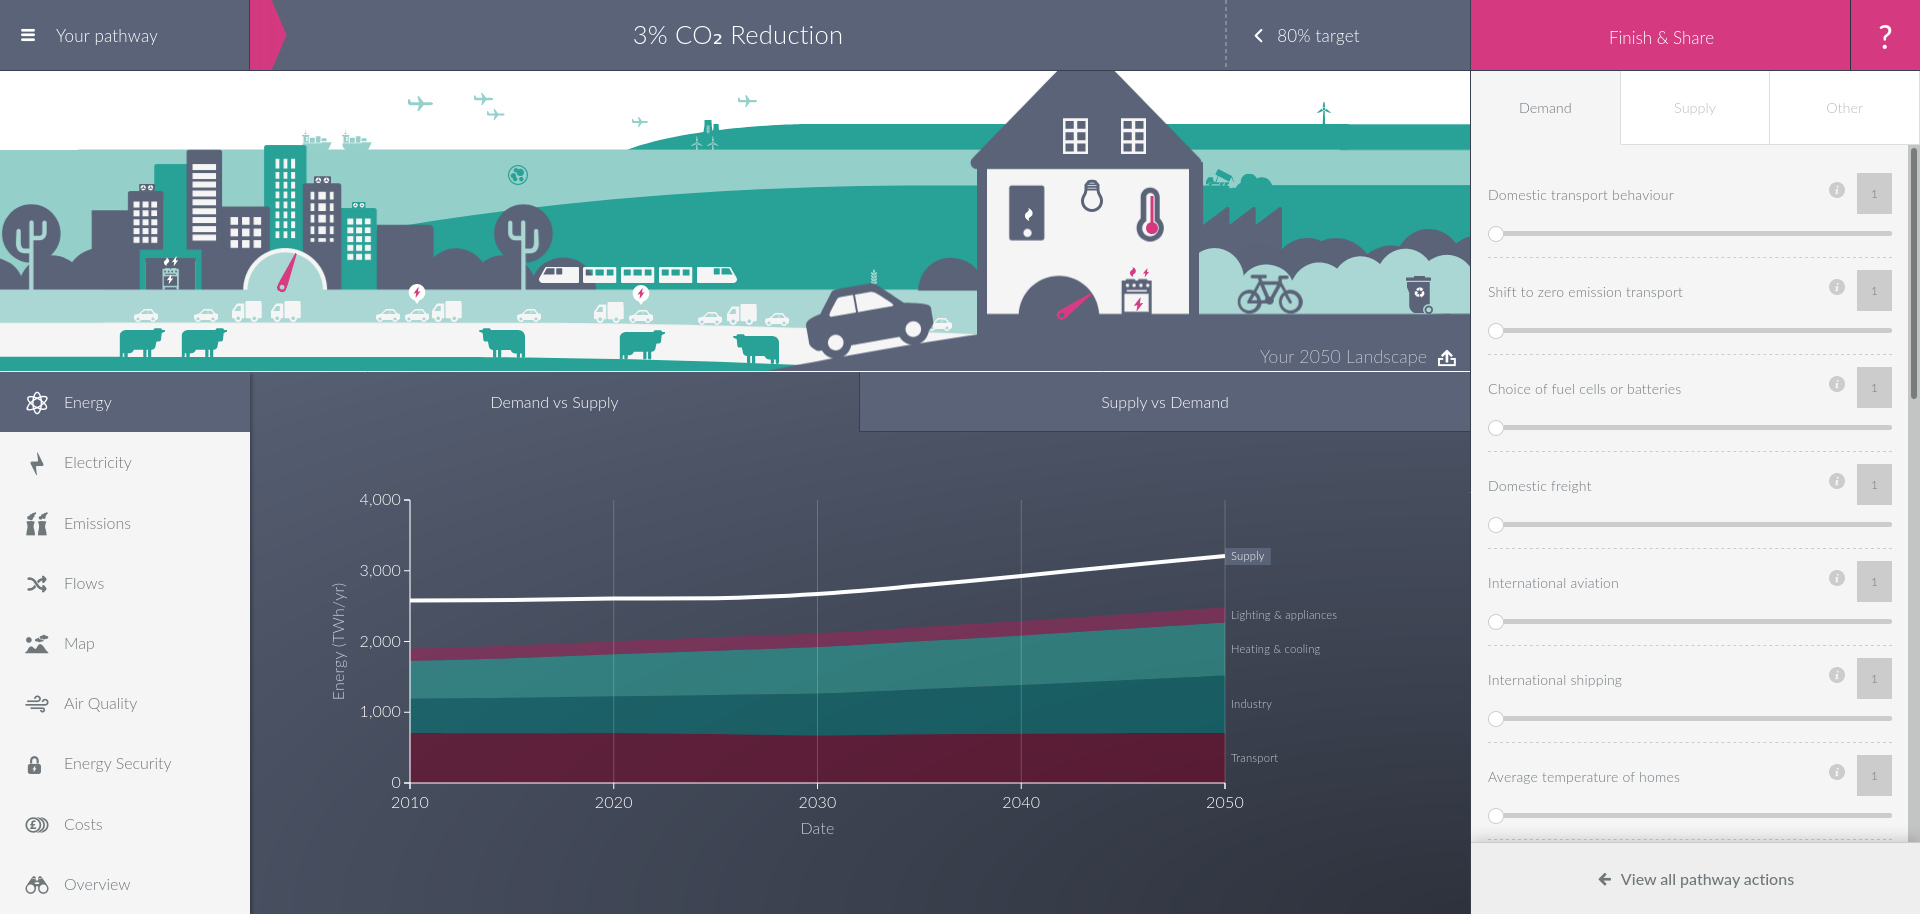
\includegraphics[height=0.24\textwidth]{files/Model_photo_3.png}
	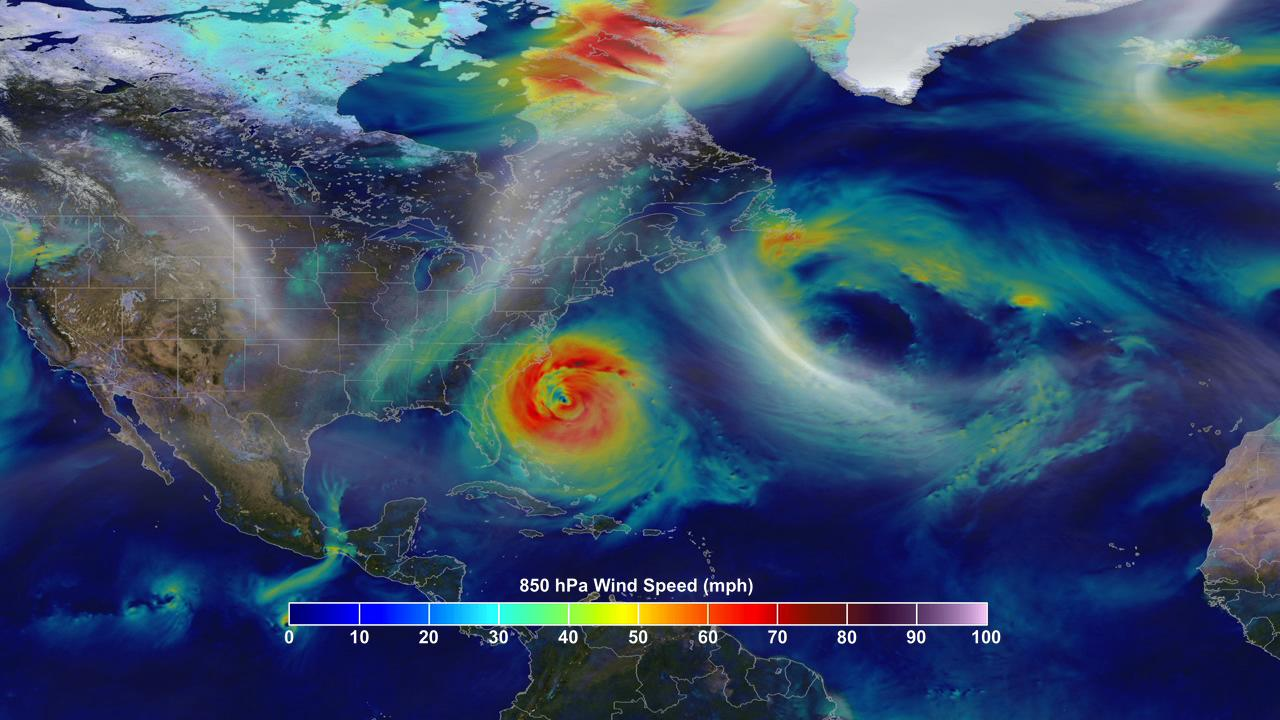
\includegraphics[height=0.24\textwidth]{files/Model_photo_4.jpg}
	\caption[Images showing different objects and/or models.]{Images showing different objects and/or models. Bottom left graphic, \copyright Leonhard Hofbauer, 2021, based on DECC released under a CC-BY-4.0, the remaining images, clockwise, are from LibraryArchives, Conal Gallagher, and NASA Goddard, respectively, and all licensed under a CC-BY-2.0}
	\labfig{model_photos}
\end{figure}

An \textbf{energy system model} is a model that depicts the energy system or at least parts of it. One could count some physical models, e.g., a small wind turbine model that is used to study design aspects, as energy model. Yet, this course focuses on computer-based energy system models that depict larger parts of the energy system (and are thus very difficult or impossible to build in a useful way as a physical model).

% TODO: add side note with more information on computer-based models

\section{The purpose of energy system models}


\paragraph{Energy models for energy planning.}~\\

Energy system models can have very different purposes but many of them are developed to support energy planning. Energy planning is the process of developing a plan with regard to the energy system for future years. Governments, companies, consumers, and many others all have to take decisions which rely on a plan for the energy future in one way or another. Have a look at the task below for one example.


\begin{kaobox}[frametitle=Task]
A local authority has to replace its entire fleet of diesel vans which are used as maintenance vehicles and for other council services. The vans can be separated in three different groups based on their usage profile. The table below  gives information about the number of vans in each group and the respective usage profile.


\begin{tabular}{ c c m{4cm} }
	\toprule
	Group & Number of vans & Distance driven per van and year (km)\\
	\midrule
	Maintenance vans & 10 & 25000\\
	Event vans & 8 & 8000 \\ 
	Other vans & 15 &20000  \\
	\bottomrule
\end{tabular}


The local council considers three different options for replacement of the fleet: the current type of diesel vans, electric vans, and biodiesel vans. The table below shows all the characteristics of the different types of vans.

\begin{tabular}{ c m{1.5cm} m{1.5cm} m{2cm} m{2cm} }
	\toprule
	Type & Capital cost (\pounds) & Lifetime (years) & Variable cost (incl. fuel) (\pounds /km)& CO$_2$ emissions (g/km)\\
	\midrule
	Diesel & 25000 & 20 &  0.08 & 300\\
	Electric & 35000 &  20 &  0.05 & 50 \\ 
	Biodiesel & 25000 & 20 &  0.10 & 100\\
	\bottomrule
\end{tabular}

How many vans of each type should the council buy if they want to minimize their annual cost but also reduce the annual CO$_{2}$ emissions from their fleet by at least 82\%? Work together in groups.\\
Tip: You can calculate the annual cost for a van in this simplified manner:\\
$ AnnualCost = CapitalCost/Lifetime + AnnualDistanceDriven \cdot VariableCost$.
\end{kaobox}

Energy planning can be a very complex task and involve questions which are very challenging to answer. Many of these questions cannot precisely be answered -- nobody knows for certain about the future -- but energy models can help us to get some answers and to think about the future in a structured way. They have been used to support decisions by the UK government, by companies, and by consumers. Because the energy system is very complex, ranging from local to global, from half-hourly to decade-long, no single model can answer all questions but many different ones are necessary to help different organisations with different energy planning questions.

% TODO: potentially add a table with different institutions, what decisions with regard to the energy system they need to take, and what underlying questions exist


\section{Different types of energy system models}

\paragraph{Differentiating energy system models.}~\\


As discussed earlier, there are a lot of different kind of energy system models with different purposes. \reftab{mclass} shows a few different characteristics we can look at when describing a particular model, along with a few potential values.~\\

% TODO: potentially add a definition of classification in a side note

\begin{table}[!t]
\caption[Classification of energy models.]{A number of different characteristics by which energy systems can be differentiated. Adapted from \cite{hall_review_2016}.}
\labtab{mclass}
\begin{tabular}{c c c }
\toprule
\bfseries Analytical approach  & \bfseries Methodology & \bfseries Sectoral coverage \\
\toprule
Top-Down  & Optimization & Whole energy system \\
Bottom-up & Simulation & Power sector  \\
Hybrid & Agent-based & Transport sector \\
Other& Econometric & Heat sector   \\
& ... & ... \\
\midrule
\bfseries Geographic coverage & \bfseries Time horizon &  \bfseries Time resolution\\
\midrule
Global &  Short term & Minute \\
National &  Medium term  & Hour \\
Regional &  Long term & Month\\
Local & & Year \\
... & & ...\\
\bottomrule
\end{tabular}
\end{table}

\begin{kaobox}[frametitle=Task]
In groups of three, come up with an energy planning question or problem and with what kind of model you could help to answer it:
\begin{itemize}
\item Think about one organization, e.g., the national government, a local authority, or a company, and what kind of question or problem they might face with regard to the future energy system. Write down the problem or question in 1-2 sentences.
\item Think about what kind of model might be appropriate to support the organization in their energy planning. You can use the classification in \reftab{mclass} to describe your model. Think about why you make your choices and note down the characteristics of your model.
\end{itemize}
Afterwards, your group needs to present your results, i.e., what organization you considered, what problem or question they might face, and what kind of model would be appropriate and why.
\end{kaobox}

    
\section{Homework}

% TODO: add more information about net-zero in a side note

In 2020, the UK government has published a simple, web-based energy model that can be used to explore pathways for the UK energy system towards its net-zero target in 2050. This is the successor of a similar tool called DECC 2050, which has been used widely by researchers, government, and other stakeholders.

The model (or calculator) has a normal and a detailed version which you can find here

\begin{itemize}
\item \href{https://my2050.beis.gov.uk/}{https://my2050.beis.gov.uk/} (normal)
\item \href{https://mackaycarboncalculator.beis.gov.uk/}{https://mackaycarboncalculator.beis.gov.uk/} (detailed)
\end{itemize}

Choose either the normal or detailed model and build a pathway that meets the government's net-zero target for 2050! Share your pathway with everybody through the virtual learning platform (once you are done creating your pathway, simply copy the current web address from the browser - it should look like this \textit{https://my2050.beis.gov.uk/?levers=1112 [...]} or this \textit{https://mackaycarboncalculator.beis.gov.uk/overview/emissions-and-primary-energy-consumption/?levers=1111 [...]}, depending on the calculator, and send it as a message to everyone) and have a look at the scenarios your classmates created. Be ready to discuss  your pathway and experience with the model in the next session.
\setchapterpreamble[u]{\margintoc}
\chapter{Power System Modelling}
\labch{psm}

After completing this session successfully, you should be able

\begin{itemize}
\item to explain the basic working principles of the power system,
\item to understand the structure of a power system model investigating the integration of variable renewable energies, and
\item  to analyse the influence of assumptions on model-based analysis results.
    
\end{itemize}

\section{The BEIS 2050 calculator}


\begin{kaobox}[frametitle=Task]
Discuss your experiences of using the BEIS calculators with your classmates and your course leader! Did you find the model straightforward to use? Was it easy to get to net zero? Did classmates come up with different but equally possible pathways you had not thought of?
\end{kaobox}

\section{How does the power system work?}


\paragraph*{The structure of a power system.}

\begin{figure}[hb]
	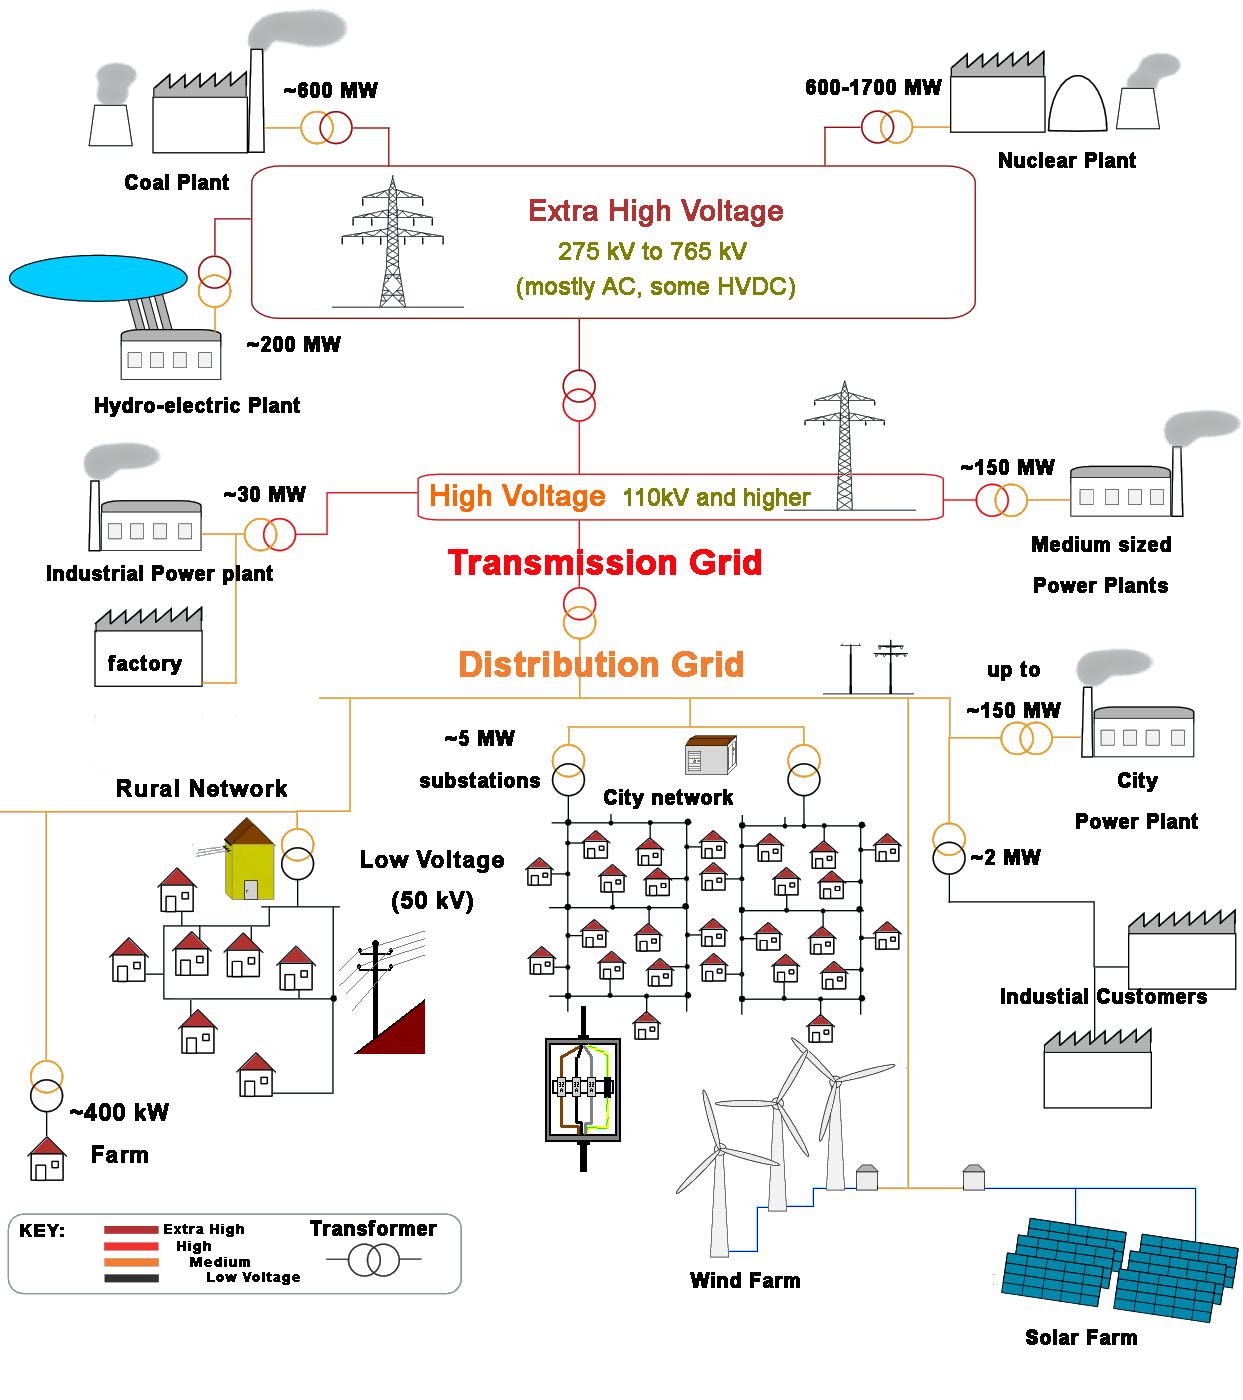
\includegraphics[width=0.8\textwidth]{files/power_system.jpg}
	\caption[Schematic diagram of the power system.]{Schematic diagram of the power system. From Quark64, licensed under a CC-BY-3.0}
	\labfig{ps}
\end{figure}

\begin{kaobox}[frametitle=Task]
Have a look at \reffig{ps}. What three different types of elements of a power system can you identify? How is the system changing now and in future?
\end{kaobox}


\begin{definition}
\labdef{eps}
An electric power system is a network of electrical components that is deployed to supply, transmit, and use electric power for various purposes \sidecite{qazi_chapter_2017}. It consists of three types of elements that
\begin{itemize}
\item generate electricity,
\item transfer electricity (transmission \& distribution), or
\item use electricity.
\end{itemize} 
\end{definition}



\paragraph*{Balancing a power system.}


\begin{kaobox}[frametitle=Task]
One could say our \textit{apple system} is very similar: there are generators, i.e., farms where apples grow, a transfer system, i.e., vans transporting apples, and users, i.e., people eating apples. What are the major differences between the \textit{apple system} and the power system?
\end{kaobox}

A very important characteristic of power systems, especially when considering future renewable and sustainable power systems, is the balance of supply and demand. In contrast to other commodities, e.g., apples, electricity cannot be stored easily. For the power system to be operated in a stable manner, the generation and consumption of electricity in a power system need to be balanced in every moment. That is, the demand of electricity in a certain second, e.g., from a kettle, needs to be matched by power plants generating the same amount of electricity in that same second, e.g., from a wind turbine.


\section{How does a power system model look like?}


% TODO: potentially add more information on structure/equations, input data/data sources/assumptions with regard to power system models

\paragraph*{Building a power system model.}
\begin{kaobox}[frametitle=Task]
A remote mountain cottage in the Scottish Highlands needs a new, sustainable power supply system. The electricity usage is very low but it is needed for light and a few other purposes. The electricity consumption has been measured in the past and is similar every day. The table below gives the power demand for each hour of this typical day.

% TODO: add side note explaining capacity factor

The cottage is not connected to the national electricity grid but there is space to install solar PV panels on the roof, small wind turbines next to the cottage, and a biodiesel generator. The actual generation of the PV panels and wind turbines depends on the weather and the table below gives the capacity factor for solar panels  $CF_S$  and wind turbines $CF_W$ for each of the hours.



\begin{tabular}{ c c c c }

	\toprule
	Hour(s) & Demand (kW) & $CF_W$ (-) & $CF_S$ (-) \\
	\midrule
	00:00 $\rightarrow$ 08:00 & 0 & 0.4 & 0.0\\
	08:00 $\rightarrow$ 09:00 & 0 & 0.3 & 0.1\\
	09:00 $\rightarrow$ 10:00 & 0 & 0.2 & 0.3\\
	10:00 $\rightarrow$ 11:00 & 2 & 0.1 & 0.5\\
	11:00 $\rightarrow$ 12:00 & 4 & 0.0 & 0.7\\
	12:00 $\rightarrow$ 13:00 & 3 & 0.2 & 0.9\\
	13:00 $\rightarrow$ 14:00 & 1 & 0.4 & 0.8\\
	14:00 $\rightarrow$ 15:00 & 0 & 0.5 & 0.7\\
	15:00 $\rightarrow$ 16:00 & 2 & 0.6 & 0.55\\
	16:00 $\rightarrow$ 17:00 & 1 & 0.7 & 0.2\\
	17:00 $\rightarrow$ 18:00 & 3 & 0.6 & 0.1\\
	18:00 $\rightarrow$ 19:00 & 5 & 0.7 & 0.0\\
	19:00 $\rightarrow$ 20:00 & 1 & 0.6 & 0.0\\
	20:00 $\rightarrow$ 24:00 & 0 & 0.3 & 0.0\\
	\bottomrule
\end{tabular}\\


\textbf{Part 1:} Two different engineering consultancy companies develop suggestions for the power supply system of the mountain cottage. Consultancy A suggests to install 2 kW of solar PV, 10 kW of wind turbines, and a 1.5 kW biodiesel generator as backup. Company B suggests to install 4 kW of solar PV, 6 kW of wind turbines, and a 2 kW biodiesel generator. Check if the suggested power supply systems would be able to satisfy the power demand on the mountain cottage! You can use the table below for your calculations.

\begin{tabular}{ c c c c c c c }

	\toprule
	& \multicolumn{3}{c}{Consultancy A}& \multicolumn{3}{c}{Consultancy A}\\
	Hour(s) & $G_W$ & $G_S$ & $G_B$  & $G_W$  & $G_S$  & $G_B$   \\
	& \multicolumn{6}{c}{(kWh)}   \\
	\midrule
	00:00 $\rightarrow$ 08:00 & \line(1,0){14}& \line(1,0){14} & \line(1,0){14} & \line(1,0){14}& \line(1,0){14} & \line(1,0){14}\\
	08:00 $\rightarrow$ 09:00 & \line(1,0){14}& \line(1,0){14} & \line(1,0){14} & \line(1,0){14}& \line(1,0){14} & \line(1,0){14}\\
	09:00 $\rightarrow$ 10:00 & \line(1,0){14}& \line(1,0){14} & \line(1,0){14} & \line(1,0){14}& \line(1,0){14} & \line(1,0){14}\\
	10:00 $\rightarrow$ 11:00 & \line(1,0){14}& \line(1,0){14} & \line(1,0){14} & \line(1,0){14}& \line(1,0){14} & \line(1,0){14}\\
	11:00 $\rightarrow$ 12:00 & \line(1,0){14}& \line(1,0){14} & \line(1,0){14} & \line(1,0){14}& \line(1,0){14} & \line(1,0){14}\\
	12:00 $\rightarrow$ 13:00 & \line(1,0){14}& \line(1,0){14} & \line(1,0){14} & \line(1,0){14}& \line(1,0){14} & \line(1,0){14}\\
	13:00 $\rightarrow$ 14:00 & \line(1,0){14}& \line(1,0){14} & \line(1,0){14} & \line(1,0){14}& \line(1,0){14} & \line(1,0){14}\\
	14:00 $\rightarrow$ 15:00 & \line(1,0){14}& \line(1,0){14} & \line(1,0){14} & \line(1,0){14}& \line(1,0){14} & \line(1,0){14}\\
	15:00 $\rightarrow$ 16:00 & \line(1,0){14}& \line(1,0){14} & \line(1,0){14} & \line(1,0){14}& \line(1,0){14} & \line(1,0){14}\\
	16:00 $\rightarrow$ 17:00 & \line(1,0){14}& \line(1,0){14} & \line(1,0){14} & \line(1,0){14}& \line(1,0){14} & \line(1,0){14}\\
	17:00 $\rightarrow$ 18:00 & \line(1,0){14}& \line(1,0){14} & \line(1,0){14} & \line(1,0){14}& \line(1,0){14} & \line(1,0){14}\\
	18:00 $\rightarrow$ 19:00 & \line(1,0){14}& \line(1,0){14} & \line(1,0){14} & \line(1,0){14}& \line(1,0){14} & \line(1,0){14}\\
	19:00 $\rightarrow$ 20:00 & \line(1,0){14}& \line(1,0){14} & \line(1,0){14} & \line(1,0){14}& \line(1,0){14} & \line(1,0){14}\\
	20:00 $\rightarrow$ 24:00 & \line(1,0){14}& \line(1,0){14} & \line(1,0){14} & \line(1,0){14}& \line(1,0){14} & \line(1,0){14}\\
	\bottomrule
\end{tabular}\\

The table below gives the relevant cost parameters for the three power generation technologies

\begin{tabular}{ c m{2.5cm} m{2.5cm} m{2cm} }
	\toprule
	Technology & Annualized capital cost (\pounds/kW) & Variable cost (incl. fuel) (\pounds /kWh) & Efficiency (-)\\
	\midrule
	PV & 49 & 0 &  1 \\
	Wind & 75 &  0 &  1 \\ 
	Biodiesel & 141 & 0.015 &  0.6 \\
	\bottomrule
\end{tabular}

\textbf{Part 2:} What is the cost-optimal power supply system for the mountain hut? Solve this together with your course leader using a power system model.
\end{kaobox}



\paragraph*{Reflecting on power system models.}~\\


As discussed in \refsec{models}, models are always a simplification of reality built for a particular purpose. Thus, it is always important to make sure the model is fit for the specific purpose it is used for and that one does not draw conclusions from model results that cannot be justified. Moreover, it is also crucial to be aware of and acknowledge the weaknesses of the models and model-based analysis.

\begin{kaobox}[frametitle=Task]
Think about the analysis with regard to the mountain cottage above. Do you think the model is based on realistic assumptions? What are the weaknesses of the analysis?
\end{kaobox}



\section{Homework}
In order to develop useful models, it is important to have a good understanding of the system to be modelled. Perform a short literature research on highly renewable power systems using a scientific search engine (for example, \href{https://scholar.google.com/}{https://scholar.google.com/}. Try to find at least 3 relevant publications, e.g., journal papers or reports, read (at least) the respective abstracts, and write a short summary of around 150-200 words. You can touch on one or more of following points (you do \textbf{not} need to cover all of them):
\begin{itemize}
\item What are the challenges associated with highly renewable power systems?
\item What are potential solutions to address those challenges?
\item What other developments within the power sector play a role?
\end{itemize}

Make sure that you use references to point to your sources. 

% TODO: add side note or otherwise more information on referencing in the handbook

\setchapterpreamble[u]{\margintoc}
\chapter{Energy System Scenarios}
\labch{ess}

After completing this session successfully, you should be able

\begin{itemize}
    \item to explain what scenarios are and how they are used,
    \item to work with a spreadsheet-based power system model, and
    \item to be able to interpret modelling results.

\end{itemize}


\section{Power sector model}

\paragraph*{Island energy planning and power sector modelling.}
\begin{kaobox}[frametitle=Task]
You have been asked to support local authorities in the planning for a future renewable power system for a remote island. Make yourself familiar with the provided framework of a power sector model together with your course leader.
\end{kaobox}


\section{Scenario analysis}

% TODO: add side note on forecast and weather forecast as example

Models can play various roles when supporting decision-making.  Some, in particular short-term models, can be used to provide \textit{forecasts}, e.g, for the electricity price of the following day. But if decision-makers are interested in long-term strategies as it is mostly the case in energy planning, using models to produce forecast is generally not useful. Planning energy systems usually happens over several decades, with many future uncertainties, from the cost of technologies, to the impact of climate change, to the behaviour of all of us who can shape the future energy system development. Thus, models for energy planning are usually not used to create forecasts, i.e., how the future \textit{will be}, but to create scenarios, i.e., how the future \textit{could be} under certain circumstances. Scenarios are descriptions of potential futures. They can have qualitative elements, i.e., a textual description, and quantitative elements, i.e., a numerical description, for example, graphs. They describe plausible future developments and can help us to explore and think about potential futures. For example, it can support decision-makers in thinking about which might be a preferable energy system and what needs to be done to achieve it.\cite{mcdowall_reflecting_2014}


\begin{kaobox}[frametitle=Shared socioeconomic pathways (SSPs) - Narratives (adopted from \cite{riahi_shared_2017} under CC-BY-4.0), backgroundcolor=Goldenrod!45!white,frametitlebackgroundcolor=Goldenrod!45!white]
\paragraph*{Sustainability – Taking the Green Road.}The world shifts gradually, but pervasively, toward a more sustainable path, emphasizing more inclusive development that respects perceived environmental boundaries. Management of the global commons slowly improves, educational and health investments accelerate the demographic transition, and the emphasis on economic growth shifts toward a broader emphasis on human well-being. Driven by an increasing commitment to achieving development goals, inequality is reduced both across and within countries. Consumption is oriented toward low material growth and lower resource and energy intensity.

\paragraph*{Regional Rivalry – A Rocky Road.}A resurgent nationalism, concerns about competitiveness and security, and regional conflicts push countries to increasingly focus on domestic or, at most, regional issues. Policies shift over time to become increasingly oriented toward national and regional security issues. Countries focus on achieving energy and food security goals within their own regions at the expense of broader-based development. Investments in education and technological development decline. Economic development is slow, consumption is material-intensive, and inequalities persist or worsen over time. Population growth is low in industrialized and high in developing countries. A low international priority for addressing environmental concerns leads to strong environmental degradation in some regions.

\paragraph*{Fossil-fueled Development – Taking the Highway.} This world places increasing faith in competitive markets, innovation and participatory societies to produce rapid technological progress and development of human capital as the path to sustainable development. Global markets are increasingly integrated. There are also strong investments in health, education, and institutions to enhance human and social capital. At the same time, the push for economic and social development is coupled with the exploitation of abundant fossil fuel resources and the adoption of resource and energy intensive lifestyles around the world. All these factors lead to rapid growth of the global economy, while global population peaks and declines in the 21st century. Local environmental problems like air pollution are successfully managed. There is faith in the ability to effectively manage social and ecological systems, including by geo-engineering if necessary.
\end{kaobox}


\begin{figure}[hb]
	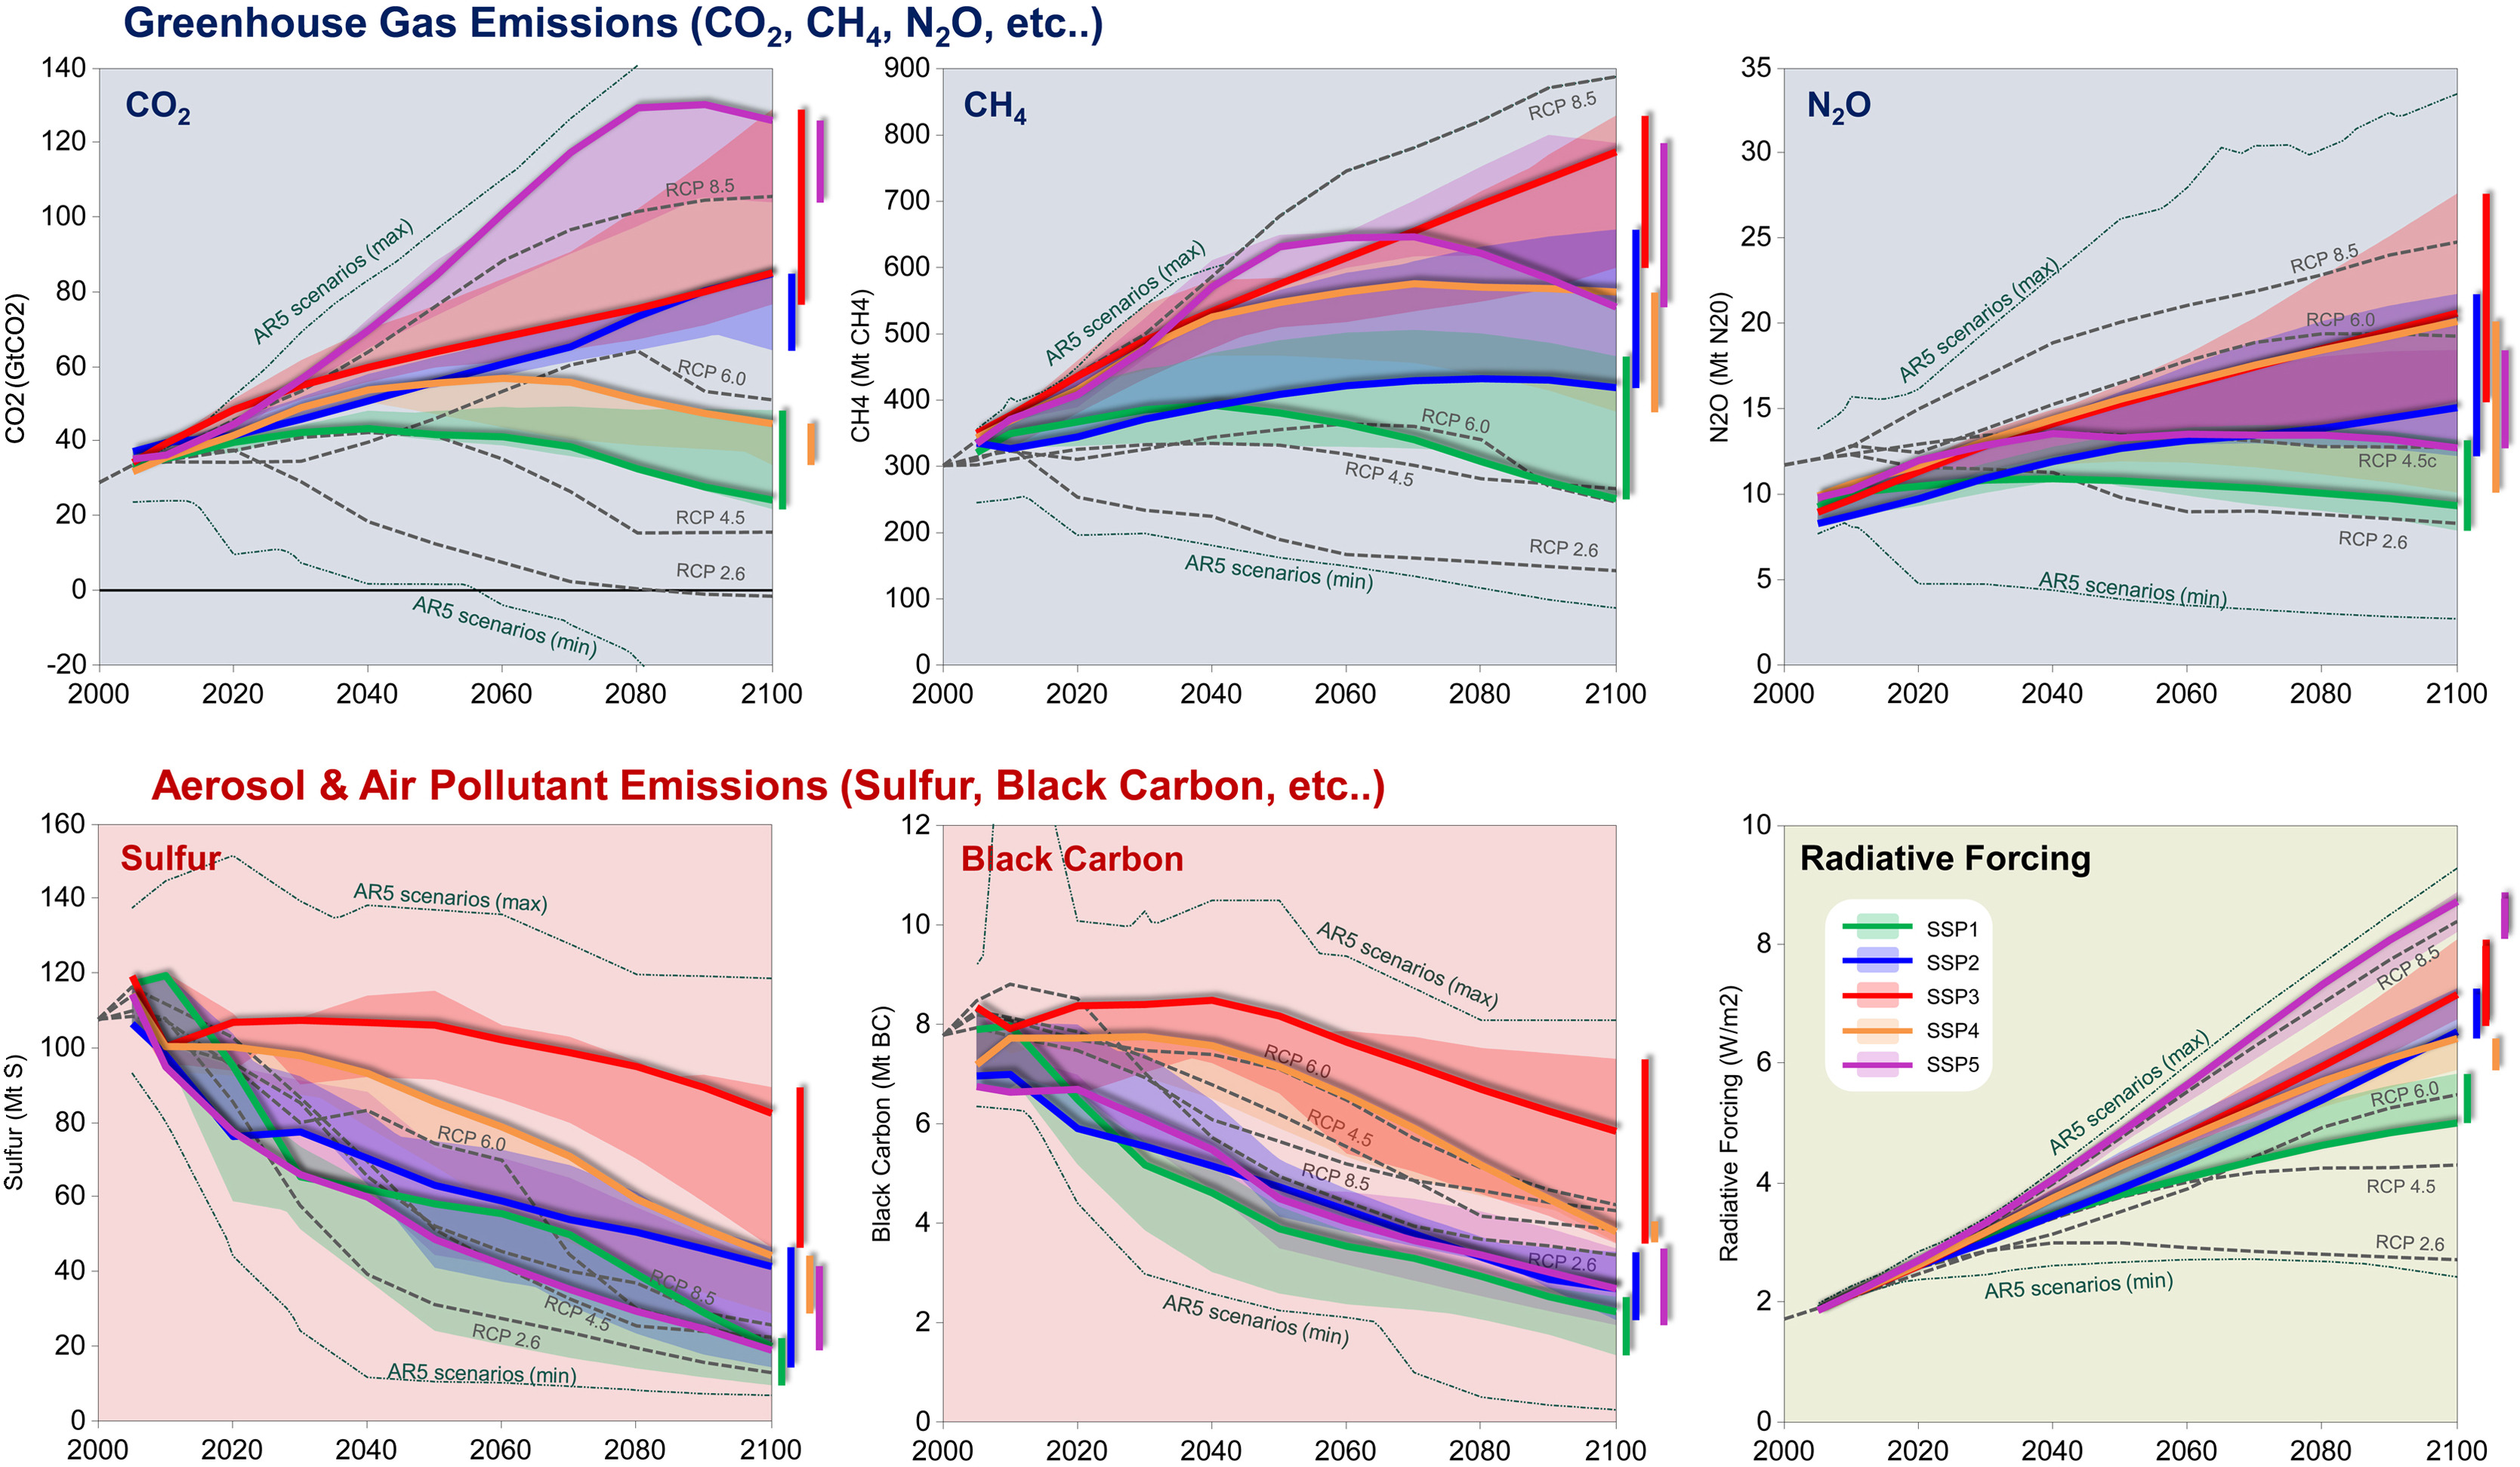
\includegraphics[width=0.98\textwidth]{files/SSP_pathways.jpg}
	\caption[Global emissions and radiative forcing for SSPs.]{Global emissions and radiative forcing for each of the SSPs. Adopted from \cite{riahi_shared_2017} under a CC-BY-4.0 license}
	\labfig{SSP_pathways}
\end{figure}

\begin{kaobox}[frametitle=Task]
Read through the qualitative narratives of the 3 (out of 5) shared socioeconomic pathways above and compare those with the quantitative emission pathways given in \reffig{SSP_pathways}. To which SSP does each of the narrative belong? Explain your choice.
\end{kaobox}


% TODO: potentially add another (optional) exercise for pupils to write one or two scenario for, e.g., the UK or the island system from before




\section{Homework}

\paragraph*{Part 1.} Have a look at and get familiar with the power sector model from the this session which will be provided by your course leader. Use the model to explore one scenario and prepare a 1-2 minute presentation of it for the next session. You can use the data already in the spreadsheet and explore this base scenario or change some of the data. You should prepare
\begin{itemize}
\item a name for the scenario,
\item a short (3-4 sentences) narrative for the scenario,
\item a short explanations of the model results (i.e., what power generation technologies will be used),
\item a short (1-2 sentences) conclusion for local policy-makers (i.e, what does the scenario tell them)
\end{itemize}


You do not need to submit this beforehand (but if you want, you can and your course leader will provide feedback) but, as said above, be prepared to present your scenario to your course leader and fellow students in 1-2 minutes.

\paragraph*{Part 2.} Think about which local area (town, city, small island, etc.) you want to help plan a renewable power system in your final assignment. Your course leader will ask for this in the next session to be able to provide you with the correct data for your power system model.
\setchapterpreamble[u]{\margintoc}
\chapter{Model-based Analyses}
\labch{ana}

After completing this session successfully, you should be able

\begin{itemize}
    \item to present a power system analysis to an audience,
    \item to recognize about the limitations of energy models, and
    \item to structure a model-based energy analysis.
\end{itemize}

\section{A first power system scenario}
\begin{kaobox}[frametitle=Task]
Present your power system scenario in 1-2 minutes to your course leader and fellow students! Incorporate all the aspects mentioned in the homework task of session 4.
\end{kaobox}


\section{Limitations of model-based analysis}
\labsec{lim}

\paragraph*{Limitations of energy modelling studies}~\\

Power sector models and other energy models can be very important tools that provide quantitative, i.e., numerically-oriented, insights for energy planning activities of decision-makers. But model-based studies also have their limitations which are important to acknowledge. Limitations depend on the model and the purpose it is used for but a few general points to consider are
\begin{itemize}
\item the aspects of the real system that are not captured in the model,
\item the boundaries of the system the model captures, e.g., geographic areas or sectors that are linked to the system but not directly represented in the model,
\item elements of the system that are only captured in a simplified manner in the model, and
\item uncertainties when building models that consider the future.

\end{itemize}

It is important to consider and acknowledge these limitations to be able to provide a justifiable and well-substantiated analysis.


\begin{kaobox}[frametitle=Task]
Consider again the power sector model introduced in the previous session and used for the very short analysis for your homework. What limitations does the model and analysis have? Go through the list above with your neighbour and note down all limitations you can think of.
\end{kaobox}

\section{Analysing and discussing results}
\labsec{res}
When analysing model results and drawing and communicating conclusions based on them, it is important to take into account the structure and data inputs of the model, as well as related limitations. As discussed in previous sessions, models are often, in particular when they consider complex energy systems, a stark simplification of reality, designed for a particular purpose, e.g., to address a particular set of questions. Hence, it is crucial to reflect about how to interpret model results and what conclusions can be drawn and which not.


\begin{kaobox}[frametitle=Task]
Imagine a study looking at a power system for Greater London is performed using the simple power sector model spreadsheet introduced in the last session. The analysis introduces two different scenarios for the year 2035. Which of the following statements/conclusions could be realistically drawn from the model results, which rather not? If not, why?

\begin{itemize}
\item In 2035, there will be 100 MW of PV panels installed on rooftops in London.
\item In scenario A, the installed capacity of PV panels reaches 100 MW in 2035.

\item The results indicate that solar panels can play a larger role than wind power in supplying power to London.
\item The results show wind turbines are cheaper than solar panels.

\item To implement the power system for scenario A the Greater London Authority will have to spent 2 billion pounds.
\item As compared to scenario A, scenario B requires only half of the investment in power generation in London.

\item The analysis shows that the Mayor of London and other decision-makers should introduce measures to foster the uptake of solar PV.
\end{itemize}

\end{kaobox}




\section{Final course work}

\textbf{Investigate a future renewable power system in your local area by exploring two scenarios!}


\textcolor{red}{[To start with, you only need to prepare a draft of this assignment. For the draft, try to implement both of your scenarios using the model and write down bullet points for each of the sections of your report. Please submit the draft assignment before the deadline set by your course leader.]}

Your course leader will provide you with a basic power sector model for the local area you have chosen in session 4. The model will be based on a spreadsheet with the same structure as the models used during previous sessions. The model includes all necessary values and the capacity factors for wind and solar power generation specific to your chosen area. Using your knowledge from the previous sessions, apply this model to analyse two different scenarios for a future power system which only uses local renewable power resources to meet the electricity demand of your area.

To create different scenarios from the base model, you can do one or more of the following:

\begin{itemize}
\item use different capacities of installed solar PV, wind turbines, etc.
\item use different technology cost by researching estimates for the future cost of technologies
\item change the demand
\item ...
\end{itemize}


Your submission is a 2000 words long report that describes your scenario analysis for local decision-makers. Your report should include the following sections:

\begin{enumerate}
\item Introduction: You can write about your motivation to perform this analysis (Why are you planning a renewable power system?), the background, for example about the efforts your local area is already pursuing (for example, do they already have a climate target?), and the aim of your study (Who will your analysis help?). In the end of the introduction, you can also explain the structure of the rest of the report (`The report is structured as follows. In the next section [...]').
\item Methodology: In this section, you should explain the model that you are using. You can talk about the assumptions (What demand do you use? What cost data?) and about how the model works, i.e., how it considers the balance between demand and supply of electricity (What is the temporal resolution? ... ).
\item Scenarios: You can split this section into two, one for each scenario. Explain the background of your scenarios by giving a narrative/storyline (What general, qualitative assumptions do you make, e.g., is it a scenario that assumes ambitious action?). Then discuss the power system based on your modelling results (How much solar and wind power will be installed? What are the cost? What are the advantages and benefits? What are the drawbacks? ... ). Use references to other sources to support your arguments. Make sure to include the graph from the spreadsheet to present your results. Reading through your scenario description, the reader should have a good idea about this `future' you are exploring.
\item Discussion: After explaining the scenarios in the previous section, you can discuss the results here (What do the results mean for local decision-makers? How do both scenario compare? ). It would be great to put the analysis in the context of other work (you can potentially use your research for homework 3). Make sure to use references to point to the others' work you are referring to. Also, please discuss the limitations of your model and analysis (What are the simplifications of the model? What other aspects does your analysis not capture?).
\item Conclusions: Here, you should give a short summary of your analysis and some concluding remarks (What is the core message of your work to local decision-makers? ...).
\end{enumerate}


Please have the following points in mind when working on your assignment:

\begin{itemize}
\item Your assignment needs to be 2000 $\pm$ 10\% words long (the list of references and captions of figures do not count towards the word limit).
\item Make sure to use references when you refer to other people's work.
\item You need to submit your report on the learning platform introduced by your course leader. Plan to do this well before the deadline to avoid technical problems at the last minute.
\end{itemize}





\appendix % From here onwards, chapters are numbered with letters, as is the appendix convention

\pagelayout{wide} % No margins
\addpart{Appendix}
\pagelayout{margin} % Restore margins

\setchapterstyle{lines}
\labpage{appendix}
%\blinddocument


%----------------------------------------------------------------------------------------

\backmatter % Denotes the end of the main document content
\setchapterstyle{plain} % Output plain chapters from this point onwards

%----------------------------------------------------------------------------------------
%	BIBLIOGRAPHY
%----------------------------------------------------------------------------------------

% The bibliography needs to be compiled with biber using your LaTeX editor, or on the command line with 'biber main' from the template directory

\defbibnote{bibnote}{These are the references in citation order used throughout the handbook.\par\bigskip} % Prepend this text to the bibliography
\printbibliography[heading=bibintoc, title=Bibliography, prenote=bibnote] % Add the bibliography heading to the ToC, set the title of the bibliography and output the bibliography note

%----------------------------------------------------------------------------------------
%	NOMENCLATURE
%----------------------------------------------------------------------------------------

% The nomenclature needs to be compiled on the command line with 'makeindex main.nlo -s nomencl.ist -o main.nls' from the template directory

%\nomenclature{$c$}{Speed of light in a vacuum inertial frame}
%\nomenclature{$h$}{Planck constant}
%
%\renewcommand{\nomname}{Notation} % Rename the default 'Nomenclature'
%\renewcommand{\nompreamble}{The next list describes several symbols that will be later used within the body of the document.} % Prepend this text to the nomenclature
%
%\printnomenclature % Output the nomenclature

%----------------------------------------------------------------------------------------
%	GREEK ALPHABET
% 	Originally from https://gitlab.com/jim.hefferon/linear-algebra
%----------------------------------------------------------------------------------------

%\vspace{1cm}
%
%{\usekomafont{chapter}Greek Letters with Pronounciation} \\[2ex]
%\begin{center}
%	\newcommand{\pronounced}[1]{\hspace*{.2em}\small\textit{#1}}
%	\begin{tabular}{l l @{\hspace*{3em}} l l}
%		\toprule
%		Character & Name & Character & Name \\ 
%		\midrule
%		$\alpha$ & alpha \pronounced{AL-fuh} & $\nu$ & nu \pronounced{NEW} \\
%		$\beta$ & beta \pronounced{BAY-tuh} & $\xi$, $\Xi$ & xi \pronounced{KSIGH} \\ 
%		$\gamma$, $\Gamma$ & gamma \pronounced{GAM-muh} & o & omicron \pronounced{OM-uh-CRON} \\
%		$\delta$, $\Delta$ & delta \pronounced{DEL-tuh} & $\pi$, $\Pi$ & pi \pronounced{PIE} \\
%		$\epsilon$ & epsilon \pronounced{EP-suh-lon} & $\rho$ & rho \pronounced{ROW} \\
%		$\zeta$ & zeta \pronounced{ZAY-tuh} & $\sigma$, $\Sigma$ & sigma \pronounced{SIG-muh} \\
%		$\eta$ & eta \pronounced{AY-tuh} & $\tau$ & tau \pronounced{TOW (as in cow)} \\
%		$\theta$, $\Theta$ & theta \pronounced{THAY-tuh} & $\upsilon$, $\Upsilon$ & upsilon \pronounced{OOP-suh-LON} \\
%		$\iota$ & iota \pronounced{eye-OH-tuh} & $\phi$, $\Phi$ & phi \pronounced{FEE, or FI (as in hi)} \\
%		$\kappa$ & kappa \pronounced{KAP-uh} & $\chi$ & chi \pronounced{KI (as in hi)} \\
%		$\lambda$, $\Lambda$ & lambda \pronounced{LAM-duh} & $\psi$, $\Psi$ & psi \pronounced{SIGH, or PSIGH} \\
%		$\mu$ & mu \pronounced{MEW} & $\omega$, $\Omega$ & omega \pronounced{oh-MAY-guh} \\
%		\bottomrule
%	\end{tabular} \\[1.5ex]
%	Capitals shown are the ones that differ from Roman capitals.
%\end{center}

%----------------------------------------------------------------------------------------
%	GLOSSARY
%----------------------------------------------------------------------------------------

% The glossary needs to be compiled on the command line with 'makeglossaries main' from the template directory


%
%% Glossary entries (used in text with e.g. \acrfull{fpsLabel} or \acrshort{fpsLabel})
%\newacronym[longplural={Frames per Second}]{fpsLabel}{FPS}{Frame per Second}
%\newacronym[longplural={Tables of Contents}]{tocLabel}{TOC}{Table of Contents}
%
%\setglossarystyle{listgroup} % Set the style of the glossary (see https://en.wikibooks.org/wiki/LaTeX/Glossary for a reference)
%\printglossary[title=Special Terms, toctitle=List of Terms] % Output the glossary, 'title' is the chapter heading for the glossary, toctitle is the table of contents heading

%----------------------------------------------------------------------------------------
%	INDEX
%----------------------------------------------------------------------------------------

% The index needs to be compiled on the command line with 'makeindex main' from the template directory

\printindex % Output the index

%----------------------------------------------------------------------------------------
%	BACK COVER
%----------------------------------------------------------------------------------------

% If you have a PDF/image file that you want to use as a back cover, uncomment the following lines

%\clearpage
%\thispagestyle{empty}
%\null%
%\clearpage
%\includepdf{cover-back.pdf}

%----------------------------------------------------------------------------------------

\end{document}
